\documentclass{article}
\usepackage[T1]{fontenc}
\usepackage{tikz}
\usepackage{amsmath, amssymb, amsthm}

\newcommand{\SWAP}{\operatorname{SWAP}}

\begin{document}

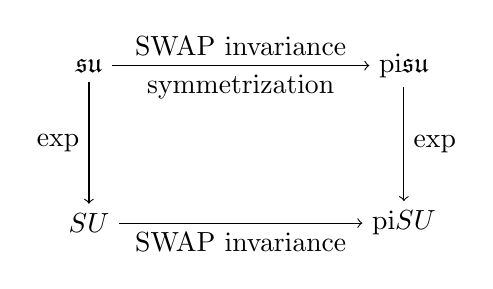
\begin{tikzpicture}[xscale = 4, yscale=-2]
    \draw (0,0) node (su) {$\mathfrak{su}$}
        (0, 1) node (SU) {$SU$}
        (1, 0) node (pisu) {$\text{pi}\mathfrak{su}$}
        (1, 1) node (piSU) {$\text{pi}SU$};
    \draw[->] (su) -- (SU) node[midway, left] {$\exp$};
    \draw[->] (su) -- (pisu) node[midway, above] {$\SWAP$ invariance} node[midway, below] {symmetrization};
    \draw[->] (pisu) -- (piSU) node[midway, right] {$\exp$};
    \draw[->] (SU) -- (piSU) node[midway, below] {$\SWAP$ invariance};
\end{tikzpicture}

\end{document}